\documentclass{article}
\author{
    Epidemiological Modelling Unit,
    \\ School of Public Health and Preventive Medicine,
    \\ Monash University
}
\usepackage{graphicx}
\usepackage[style=nature, backend=biber]{biblatex}
\usepackage{threeparttable}
\usepackage{tabularx}
\usepackage[left=2.5cm,right=2.5cm,bottom=2.5cm]{geometry}
\usepackage[singlelinecheck=false,justification=justified,labelfont=bf]{caption}
\setlength{\belowcaptionskip}{-10pt}

\addbibresource{../../references/emu_library.bib}
\title{Modelling methods, Kiribati application}

\begin{document}
\linespread{1.25}

\maketitle
\tableofcontents
\newpage
% This file describes the general structure of some of our tb_dynamics models.

\section{Model Structure}

\subsection{General features}

We use a deterministic compartmental model including six types of compartments that represent 
different states of infection and disease. The model uses the same conceptual approach and similar 
assumptions to previously published models \cite{trauer-2017, ragonnet-2019, ragonnet-2021, ragonnet-2022}. 
Here we describe the model structure without treatment compartment and related factors. 
\newline
A susceptible compartment (S) is used to represent individuals who have 
never been infected with \emph{Mycobacterium tuberculosis (M.tb)}. Latent TB infection (LTBI) is modelled 
using two successive compartments: early latent (E) and late latent (L) to capture the declining risk of 
disease progression over time from infection \cite{ragonnet-2017}. The active disease compartment (I) represents 
individuals who have progressed to the active stage of TB disease. Diseased individuals who recover 
through self-cure progress directly to the recovered compartment (R).
\newline
Non-TB-related mortality is modelled by applying death rates to all model compartments. In addition, 
disease-specific mortality is implemented by applying increased mortality rates to the active disease 
compartments (I).
\newline
Reinfection occurs in the model in two different ways. First, latently infected individuals may be 
reinfected, with this process modelled using a flow from the late latent (L) to the early latent 
compartment (E). Second, individuals who have recovered from TB disease may be reinfected and 
return to the early latent compartment. The structure of our model allows for differential risk of 
infection for the currently and previously infected individuals, compared to the infection-naive 
individuals.
\begin{figure}[!htp]
    \vspace*{-1cm}
    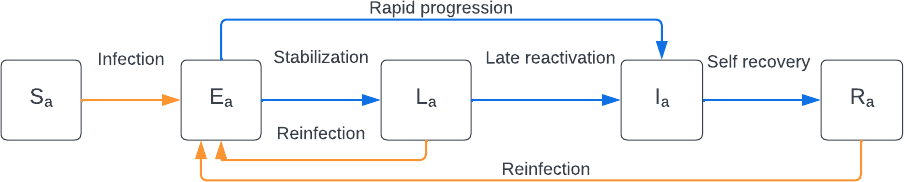
\includegraphics[width=\textwidth,height=\textheight,keepaspectratio]{images/model.png}
    \caption{Illustration of the model structure. 
    Boxes represent the different compartments types: susceptible (S), early latent (E), late latent (L), infectious (I), and recovered (R).
    The subscript indicates that compartments are stratified by age (a).}
    \label{fig:model}
\end{figure}

\subsection{Stratification by age}
The model is stratified using five categories: 0-4, 5-14, 15-34, 35-49 and 50+ years old. We assume 
heterogeneous mixing by age using an age-specific contact rate matrix. Since no local estimates of 
contact patterns by age were available for the Marshall Islands, we used a contact survey conducted in 
the Fijian population and adjusted the estimates to account for age distribution differences between
the two countries.



\section{Demographics}
\subsection{Crude birth rate and death rate}
Births are modelled using time-variant crude birth rates that are multiplied by the modelled population 
size to determine the number of newborn individuals entering the youngest age category (0 - 4) at each time. A time-variant 
and age-specific rate of non-TB-related mortality applies to all model compartments to simulate 
deaths from other causes than TB. We use estimates from the UN Population Division\footnote{https://population.un.org/wpp/Download/Standard/Mortality/} to inform the 
birth and mortality rates.
We also apply additional death rates to the compartment I to reflect mortality induced by TB 
disease.
\begin{table}[!htp]
    \caption{\textbf{Model Parameters}}
    \label{tab:parameter}
    \begin{tabularx}{\textwidth}{ X  X  c }
        \hline
        \textbf{Parameter} & \textbf{Value} & \textbf{Evidence} \\
        \hline
        \textbf{Population characteristics} & & \\
        
ISO3 code for source country for mixing matrix & GBR  & Closest demographic profile to Australia \\ 
\hline
Starting infectious seed & 2.0 persons & Arbitrary \\ 
\hline
Proportion of active period before isolation & 0.333  & Assumed \\ 
\hline
Relative infectiousness of asymptomatic persons per unit time & 0.5  & Assumed \\ 
\hline
Relative infectiousness of isolated cases & 0.2  & Assumed \\ 
\hline
Reduction in transmission risk for boosted & 0.6  & Viral load substantially lower in boosted compared to two dose vaccinated persons \cite{puhach-2022} \\ 
\hline
Reduction in transmission risk for primary course & 0.2  & Half of estimate of 40\% for Delta \cite{eyre-2022, harris-2021} \\ 
\hline
Adjustment to base case fatality rates & 0.15  & Adapted to match local epidemiology \\ 
\hline
BA.1 infection cross protection against BA.5 infection & 0.0  & No immunity from BA.1 is retained through to the BA.5 period \\ 
\hline
BA.2 infection cross protection against BA.1 infection & 1.0  & Immunity from subsequent strains is assumed to completely protect against previous strains \\ 
\hline
BA.5 infection cross protection against BA.1 infection & 1.0  & Immunity from subsequent strains is assumed to completely protect against previous strains \\ 
\hline
BA.5 infection cross protection against BA.2 infection & 1.0  & Immunity from subsequent strains is assumed to completely protect against previous strains \\
        Crude birth rate  & Time-variant & UN Population Divison \\
        Universal death rate & Time-variant & UN Population Divison \\
        \hline
        \textbf{\emph{M.tb} infection and TB} \\
        Rate of stabilization from early to late latency &    
        \begin{minipage}[t]{0.3\textwidth}
            Age 0-4: 4.4 per year \newline
            Age 5-14: 4.4 per year \newline
            Age 15+: 2 per year \newline
        \end{minipage}
        & 
        \begin{minipage}[t]{0.4\textwidth}
            Table 1, Parameter estimates. Calibration issued from the survival likelihood maximisation applied 
            to the merged dataset (Victoria and Amsterdam data), Ragonnet et al.\cite{ragonnet-2017}
        \end{minipage} \\
        Rate of rapid progression to active TB & 
        \begin{minipage}[t]{0.3\textwidth}
            Age 0-4: 2.4 per year \newline
            Age 5-14: 2 per year \newline
            Age 15+: 0.1 per year \newline
        \end{minipage}
        & 
        \begin{minipage}[t]{0.4\textwidth}
            Table 1, Parameter estimates. Calibration issued from the survival likelihood maximisation applied 
            to the merged dataset (Victoria and Amsterdam data) \cite{ragonnet-2017}
        \end{minipage}  \\
        Rate of late reactivation & 
        \begin{minipage}[t]{0.3\textwidth}
            Age 0-4: 7e\textsuperscript{-9} per year \newline
            Age 5-14: 2.3e\textsuperscript{-3} per year  \newline
            Age 15+: 1.2e\textsuperscript{-3} per year \newline
        \end{minipage}
        &
        \begin{minipage}[t]{0.4\textwidth}
        Table 1, Parameter estimates. Calibration issued from the survival likelihood maximisation applied 
        to the merged dataset (Victoria and Amsterdam data), \cite{ragonnet-2017}
        \end{minipage} \\
        Relative risk of reinfection while latently infected (ref. infection-naive) & 0.2 &
        \begin{minipage}[t]{0.4\textwidth}
        The weighted mean adjusted incidence rate of tuberculosis in the LTBI and UI 
        groups attributable to reinfection was 13.5 per 1000 person-years
        (95\% confidence interval [CI]: 5.0–26.2 per 1000 person-years) and that 
        attributable to primary infection was 60.1 per 1000 person-years 
        (95\% CI: 38.6–87.4 per 1000 person-years). \cite{andrews-2012}
        \end{minipage} \\
        Relative risk of reinfection after recovery (ref. infection-naive) & 0.2 & \begin{minipage}[t]{0.4\textwidth}
        The adjusted IRR for tuberculosis in the LTBI group compared with the UI group was 0.21. \cite{andrews-2012} 
        \end{minipage} \\
        \hline
	\end{tabularx}
\end{table}

\begin{figure}[!htp]
   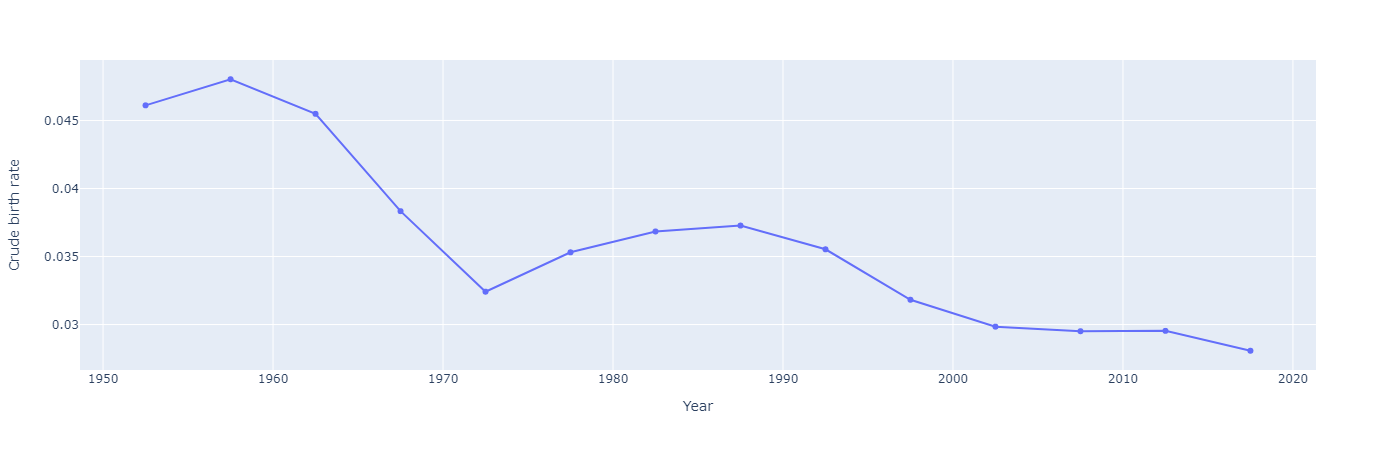
\includegraphics[width=\textwidth,keepaspectratio]{images/cbr.png}
    \caption{The crude birth rate of Kiribati from 1950 to 2020.}
    \label{fig:cbr}
\end{figure}

\begin{figure}[!htp]
   \centerline{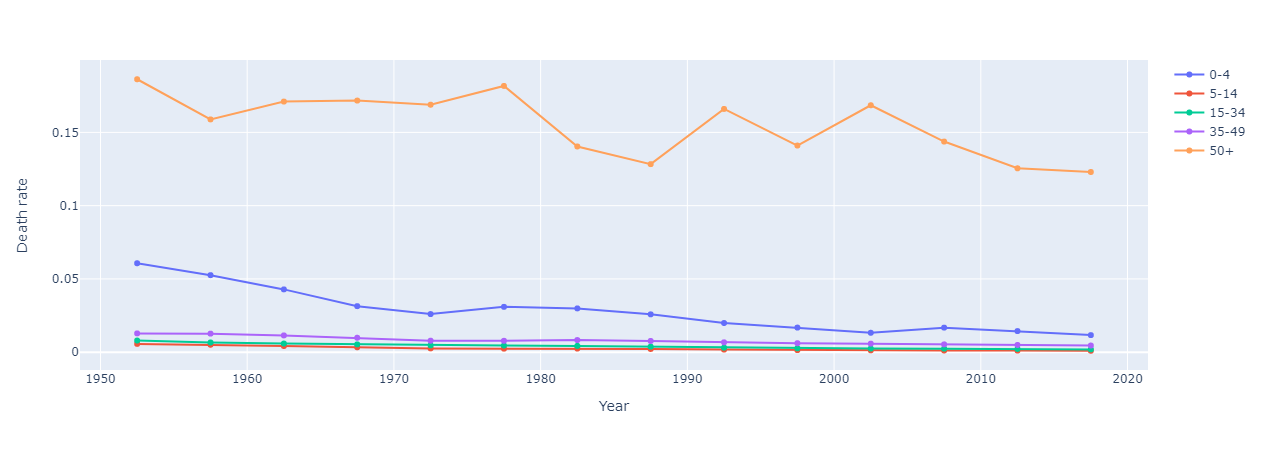
\includegraphics[width=\textwidth,keepaspectratio]{images/cdr.png}}
    \caption{The death rate of Kiribati from 1950 to 2020, stratified by age group.}
    \label{fig:cdr}
\end{figure}

\subsection{Comparing modelled population with actual population}
\begin{figure}[!htp]
    \centerline{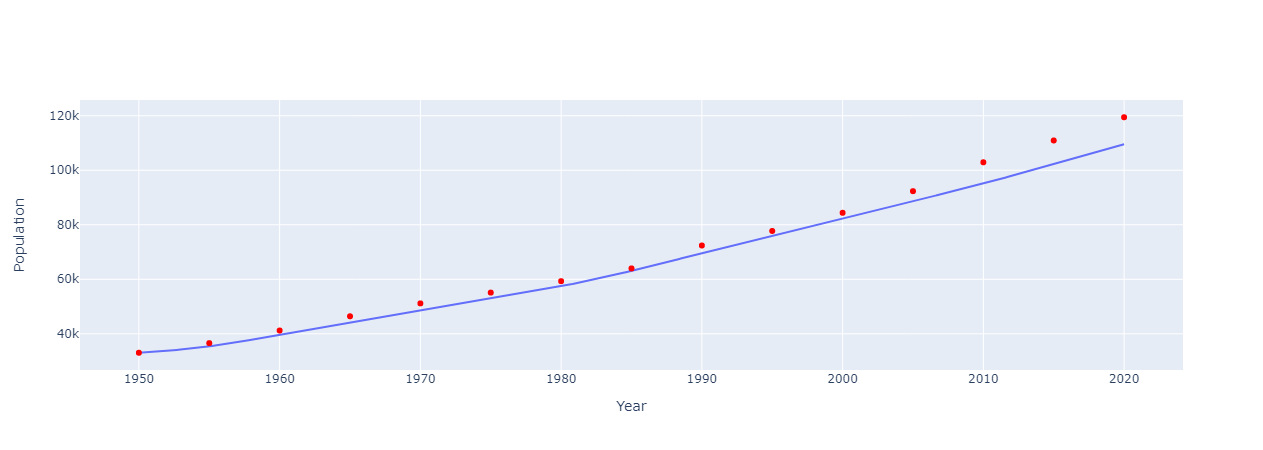
\includegraphics[width=\textwidth,keepaspectratio]{images/modelled_total.png}}
    \caption{Comparing modelled population with actual population of Kirbati from 1950 to 2020. The red dots represent the actual population size of Kiribati,
     while the blue line represents the modelled population size}
    \label{fig:modelled_total}
\end{figure}

\begin{figure}[htp]
    \centerline{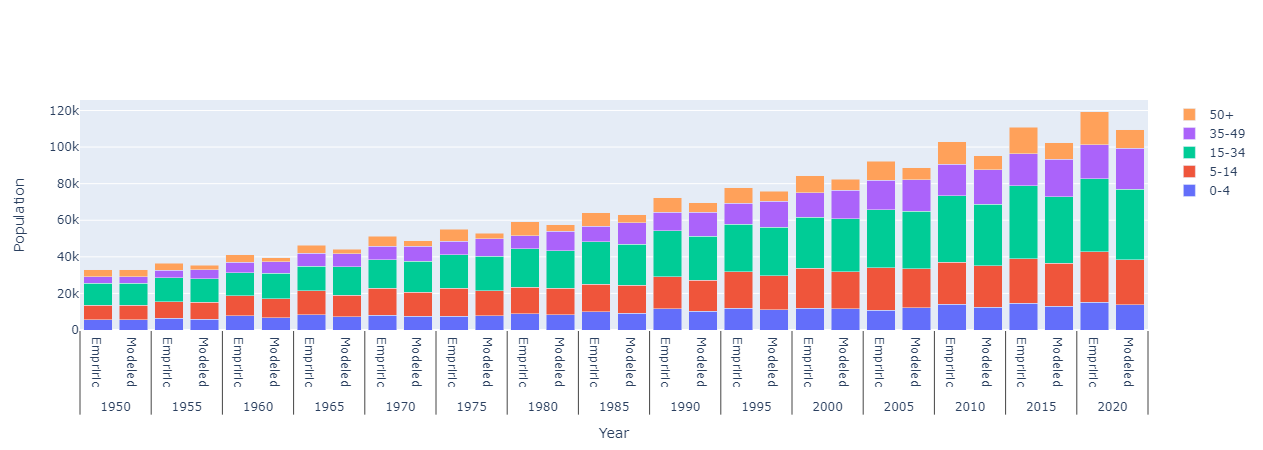
\includegraphics[width=\textwidth,keepaspectratio]{images/compare_pop.png}}
    \caption{Comparing modelled population with actual population by age groups of Kirbati from 1950 to 2020.}
    \label{fig:compare_group}
\end{figure}

\newpage    
\printbibliography
\end{document}
